
\chapter{Introduction}


Agriculture and its allied sectors in India in 2016 accounted for 15.4\%  of the GDP(Gross Domestic Product). India ranks first globally with highest net cropped area. With this big of a stretch in the economic contribution, human resource involvement of over 31\% reported in 2014 and a majority of land occupancy of around 60.45\% of the total land in India, the agricultural sector is suffering due to very little or no involvement of technology in the whole sector, among other factors. Farmers rely on rudimentary methods and intention based methodology to analyse and act upon their crop fields. There is a very little contribution of government in improving the agriculture in technical areas due to its heavy investment in solving problems like Middlemen crisis, social crisis and sudden reduction in man-power in the sector due to emergence of newer sectors and digital transformations in the country. 
\\

In our study, we focus on the areas of field analysis in the agroforestry regions to get insights on the crop field and act upon them at a larger level. The current analysis is done by farmers using a low altitude analysis with bare eyes. This results in farmers getting to check the whole field manually without any special aids and results in a raw analysis of chlorophyll  levels and thus the plant health. A very bleak section of farmers who earn enough, get the technical aids of using satellite imagery for the plant health assessment. This is a relatively newer field and costs hefty amounts of money to the farmers for even a single health monitoring, is inaccurate at miniature scales where the analysis is actually required and is mostly inaccessible in an user friendly format. This proves to be ineffective method of field analysis if done in isolation without anymore analysis and is known to only a handful of farmers.
\\

Therefore we propose a solution which could work more accurately at miniature level, reduces the manual inspection to negligible levels, is cheaper and can be made available to the farmers as a service for the complete analysis of their agricultural fields. The solution is called as Dronalyser, which is a drone based service for the agricultural inspection of the agricultural crop fields. The drone based service has the following parts:




\begin{figure}[H]
    \centering
    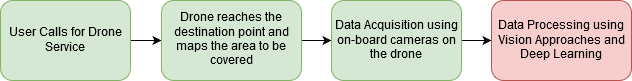
\includegraphics[width=\linewidth]{SummerInterReport/project/Images-Major/Intro_Flow.png}
    \caption{A concise flow of the proposed idea}
    \label{fig:Concise Flow}
\end{figure}

\section{Overview}

Our work compiles a study and explores various developments of a multispectral processing system based on an UAS (Unmanned Aerial System) to perform analysis on agricultural fronts to enable farmers for precision farming. The drone component covers the UAS part where it covers the area based on a service call from the application. The imagery part is achieved by an embedded system, Raspberry Pi, which does the data acquisition and data processing. A modified one camera setup of the NoIR (No InfraRed Filter CMOS sensor) camera has been tested with a Red Light Filter as well as a setup having two cameras, a normal RGB camera and a NoIR camera has also been tested for similar results. The data processing involved comparison of reflectance of NIR and Red spectra to calculate the NDVI and thereby assess the plant health.


\section{Calling for Drone Service}
We have built an android application which the user can use, either in Hindi or English, to call for the drone service. The application has an easy to use interface where the farmer's phone gets registered as a user and the farmer can call for the drone at his own position using phone's GPS. He has to further draw his field in the map provided with the application to set up the area that has to be covered by the drone for analysis. He can also use his user ID to fetch his previous reports from the Firebase storage database. The setup is made such that he can also look at the live status of the field analysis over LAN (Local Area Network) if the he is close to the drone using his phone. These can be changed to a call in case the farmer doesn't own a smartphone, in which case the service would offer a personnel for operating the drone and presenting the reports.
\section{Drone Mapping the area} The drone covers the area autonomously using geo-location based based on GPS tag from the user. We used the ArduPilot APM 2.8 flight controller which has an embedded software for GPS integration, external Compasses, I2C and even telemetry. The APM was programmed using open-source software, the firmware ArduCopter 5.3.3 uploaded through Mission Planner, which is based in ArduPilot platform to first follow the GPS tag to the Field location from the nearest Base Station and then covering the complete area through covering the polygon drawn by the farmer to cover his complete field

\section{Data Acquisition} The data acquisition system consisted of a Raspberry Pi, A NoIR Pi camera and the trigger from the APM. An open source plugin in Mission Planner, OperDroneMap(ODM) was used to merge the multi-spectral imagery into an orthomosaic from the captured images. 

\section{Data Processing} The data is processed as live time feed of the drone imagery where every frame is processed to yield the infographic feed and the post processing involves combine the individual frames into an orthomosaic covering the entire field using an open source software Fiji or using mathematical modelling of the distance. A Python script is also developed which calculates the Normalized Difference Vegetation Index (NDVI) through the Near InfraRed (NIR) and Red field reflectance spectra collected from the NoIR Pi camera, acting as a metric to define the plant health through chlorophyll level analysis. This NDVI calculation is done both on the frame wise feed and the final orthomosaic. The complete informational graphic developed lets the farmer know which areas of his field are poor in chlorophyll and thereby health. Also, we present a water index of the field using only the Near IR spectra, which is a clear indicator of water's thermal coefficient and thereby the water retention in every region of the crop field. 



